\documentclass[12pt]{article}
\usepackage{imakeidx} % Per creare un vero indice
\usepackage{amsmath}
\usepackage{booktabs}
\usepackage{verbatim}
\usepackage{listings} %Python
\usepackage{amsfonts}
\usepackage{tcolorbox}
\usepackage{titlesec}
\usepackage{ragged2e}
\usepackage{setspace}
\usepackage{caption}
\usepackage{fancyhdr}
\usepackage{listings}
\usepackage{algorithm}
\usepackage{algpseudocode}
\usepackage{hyperref}
\usepackage{tikz}
\usepackage{float}
\usepackage{array}
\usepackage{graphics}
\usepackage{multirow}
\usepackage{listings}
\usetikzlibrary{arrows}
\usepackage{graphicx} % Importa il pacchetto graphicx per l'inserimento di immagini
\usepackage{multicol} % Per avere la multicolonna
% Imposta i margini del documento
\usepackage[a4paper, top=3cm, bottom=3cm, left=3cm, right=3cm, bindingoffset=1cm]{geometry}
% Imposta il carattere Times New Roman
\usepackage{mathptmx}
\usepackage{titlesec} % Per \HRule
\definecolor{main}{HTML}{5989cf}
\definecolor{sub}{HTML}{cde4ff} 
\newcommand{\HRule}{\rule{\linewidth}{0.5mm}}

\newtcolorbox{boxC}{
	colback = sub, % background color
	boxrule = 0pt  % no borders
}

\lstset{ %
	backgroundcolor=\color{white},   % choose the background color
	basicstyle=\footnotesize,        % size of fonts used for the code
	breaklines=true,                 % automatic line breaking only at whitespace
	captionpos=b,                    % sets the caption-position to bottom
	commentstyle=\color{mygreen},    % comment style
	escapeinside={\%*}{*)},          % if you want to add LaTeX within your code
	keywordstyle=\color{blue},       % keyword style
	stringstyle=\color{mymauve},     % string literal style
}
\renewcommand{\headrulewidth}{0pt}
\setlength{\headheight}{60pt} % Altezza dell'intestazione
\setlength{\headsep}{50pt} % Distanza intestazione - contenuto

\makeindex % Indice
\begin{document}
	
	\begin{titlepage}
	\thispagestyle{fancy} % Stile fancy solo per questa pagina
	\fancyhf{} % Cancella intestazioni e piè di pagina di default
	\fancyhead[L]{
\includegraphics[width=4.5cm]{C:/Users/Denise/Downloads/logodisamis.jpg}} % Immagine a sinistra
	\fancyhead[R]{
\includegraphics[width=3cm]{C:/Users/Denise/Downloads/logounisa.png}} % Immagine a destra
		\begin{center}
			
			% Topo
			\textsc{\LARGE Università degli Studi di Salerno}\\[1.5cm]
			\textsc{\large DIPARTIMENTO DI SCIENZE AZIENDALI - MANAGEMENT \& INNOVATION SYSTEMS}\\[0.2cm]
			\textsc{\large Corso di Laurea Magistrale in Data Science \& Gestione dell'Innovazione}\\[0.2cm]
			
			% Titolo
			\HRule \\[0.3cm]
			{ \huge \bfseries Project Work PxDS}\\[0.4cm]
			\HRule \\[1.5cm]
			
			\begin{center}
				\textbf{A.A. 2024-2025} \\
				\textbf{Docente: F. Orciuoli} \\[1.5cm]
				\textbf{Gruppo N.1}\\
				\textbf{\bfseries Candidati:\\}
				\textsc{Bruno Maria Di Maio - Mat.0222800149}\\
				\textsc{Lucia Brando - Mat.0222800162}\\
				\textsc{Denise Brancaccio - Mat. 0222800163}
			\end{center}
			
		\end{center}
	\end{titlepage}
\newpage

	\tableofcontents

\newpage

	\section{Introduzione}
Questa documentazione descrive il lavoro svolto per l'esame di Programming for Data Science sviluppato dal nostro gruppo di lavoro, volto all'analisi automatizzata di discorsi politici. Dopo una panoramica della traccia assegnata, vengono presentate le tecnologie utilizzate, l'organizzazione del lavoro e le ipotesi applicative del sistema. In seguito, nei successivi capitoli, vengono illustrate le funzionalità del codice, i diagrammi di sequenza per la soluzione dei requisiti, gli esempi pratici di utilizzo e l'analisi delle prestazioni. Infine, nell'ultima sezione, vengono riportati i risultati raggiunti e i link di riferimento per la repository Github del progetto.

	\subsection{Project Work}
La traccia del progetto ha richiesto lo sviluppo di una data pipeline per l'arricchimento di un dataset chiamato speech-a.tsv, composto da tre tipi di contenuto: nomi di politici, i loro discorsi e dei un valore binario ad essi associato. L'obiettivo finale è creare un nuovo dataset che supporti l'analisi e la detection di forme di propaganda all'interno dei discorsi. L'arricchimento prevede l'integrazione di informazioni sugli autori e i loro discorsi, l'aggiunta di feature linguistiche e contenutistiche come leggibilità, sentiment, parole chiave, e narrative sottostanti, oltre alla possibilità di individuare offset e tecniche specifiche di propaganda.

	\subsection{Definizioni utilizzate}
In una prima fase, il team si è occupato dello studio e della definizione di due concetti fondamentali per lo svolgimento del lavoro: 'propaganda' e 'storytelling'. Per comprendere appieno cosa sia la propaganda, ci siamo riferiti alla seguente definizione fornita dal Dizionario di Politica di N. Bobbio, N. Matteucci e G. Pasquino (Torino, Utet Libreria, 2004, p. 775):

	\begin{quote}"La propaganda può essere definita come la diffusione deliberata e sistematica di messaggi indirizzati a un determinato uditorio, con l'obiettivo di creare un'immagine positiva o negativa di determinati fenomeni (persone, movimenti, eventi, istituzioni, ecc.) e di stimolare determinati comportamenti. La propaganda è quindi uno sforzo consapevole e sistematico volto a influenzare le opinioni e le azioni di un pubblico o di un'intera società. In questo contesto, il termine 'propaganda' viene originariamente utilizzato dalla Chiesa cattolica per indicare attività di proselitismo, senza connotazioni esplicitamente negative." \end{quote}
	
\newpage

Successivamente, è stato ampliato lo studio sulla persuasione e le tecniche di propaganda, approfondendo la lettura di testi specifici.
Lo studio condotto sulla propaganda si basa principalmente su due lavori: 'The Science of Persuasion' di Robert B. Cialdini e 'A Survey on Computational Propaganda Detection' di G. Da San Martino, S. Cresci, A. Barron-Cede, S. Yu, R. Di Pietro e P. Nakov.
Il primo paper esplicita come la persuasione sia la base della propaganda e si fondi su sei principi chiave:\\
\textbf{Validazione Sociale:} La validazione sociale può avere effetti controproducenti, ad esempio quando campagne informative evidenziano comportamenti indesiderati, portando a un aumento di tali comportamenti anziché a una loro diminuzione.\\
\textbf{Affetto:} La connessione personale e l'affetto possono aumentare la propensione a dire di sì. Complimenti e la percezione di cooperazione tra le persone possono stimolare sentimenti positivi e comportamenti favorevoli.\\
\textbf{Autorità:} L'autorità può influenzare il comportamento delle persone, come dimostrato da esperimenti in cui figure autoritarie attirano l'attenzione e inducono le persone a seguire il loro esempio.\\
\textbf{Scarsità:} La scarsità di un prodotto o di informazioni può aumentare il suo valore percepito, spingendo le persone a compiere azioni per non perdere opportunità.\\
\\
Il secondo paper, A Survey on Computational Propaganda Detection, ha offerto al team una panoramica  esaustiva sulle tecniche di rilevamento della propaganda computazionale, attraverso l'importanza di un approccio integrato che combini \textbf{l'analisi del linguaggio naturale (NLP)} e \textbf{l'analisi delle reti (Network Analysis)}.\\
Le tecniche di rilevamento della propaganda si basano principalmente sull'analisi testuale, sfruttando strumenti avanzati di NLP per identificare e classificare le tecniche propagandistiche presenti nei testi. Tra le principali attività spiccano la classificazione binaria, che determina se una frase contiene elementi propagandistici, e la classificazione multi-etichetta, che identifica frammenti testuali specifici utilizzando determinate tecniche e categorizzandoli. Modelli contestuali come \textbf{BERT} e \textbf{RoBERTa}, utilizzati all'interno del codice del progetto, si sono dimostrati particolarmente efficaci nel migliorare la precisione e l'affidabilità della classificazione.\\
\\
Un'ulteriore studio sulla propaganda e la narrativa è stato effettuato tramite il paper \textbf{Reports of personal experiences and stories in argumentation: Datasets and Analysis} di N. Faalk e G. Lapesa, Institute for Natural Language Processing, University of Stuttgart.
Il paper analizza la narrativa come un elemento essenziale dell'argomentazione e della discussione pubblica, ponendo particolare attenzione ai racconti personali e alle storie condivise dalle persone. Queste narrazioni, spesso basate su esperienze individuali e arricchite da elementi emotivi, si rivelano strumenti potenti per catturare l'attenzione, favorire l'empatia e rendere gli argomenti più accessibili e relazionabili.\\

\newpage

La ricerca ha sottolineato come le narrazioni personali possano migliorare la qualità del dibattito, aumentando la persuasività degli argomenti e facilitando la comprensione reciproca tra i partecipanti. In contesti complessi, come le discussioni su questioni sociali, le sole informazioni fattuali potrebbero non essere sufficienti a comunicare l'urgenza o l'importanza di una tematica. Le storie, in questi casi, diventano un mezzo indispensabile per costruire un dialogo più profondo e consapevole.\\ 
Queste conoscenze hanno guidato il team nello sviluppo del codice, assicurando che le soluzioni implementate tenessero conto delle dinamiche narrative e delle loro caratteristiche, per un'analisi più accurata e sensibile del contenuto testuale.

	\subsection{Organizzazione del gruppo}
	Il progetto si è svolto nell'arco di 20 giorni, con un impegno medio di circa 5 ore al giorno, seguendo una struttura collaborativa che ha ottimizzato l'assegnazione dei compiti. \\
	Bruno Maria Di Maio ha iniziato immediatamente a lavorare sui primi due punti di scraping, concentrandosi sull'aggiunta di informazioni sull'autore e dei metadati relativi ai discorsi. Lucia Brando, cooperando con Denise Brancaccio, si è occupata dei punti successivi, con un'attenzione particolare alla definizione e selezione delle feature da includere nel dataset. \\
	Successivamente, Bruno Maria Di Maio ha integrato e ottimizzato il codice, gestendo la creazione degli offset e implementando modelli di linguaggio per il trattamento avanzato del testo. Infine Denise Brancaccio, ha curato la redazione della documentazione finale, sintetizzando le scelte metodologiche e le fasi operative.\\
	Questa suddivisione ha garantito un'organizzazione efficace e ha permesso di completare il progetto nei tempi previsti, soddisfacendo i requisiti richiesti dalla traccia.
	
	\subsection{Tecnologie utilizzate}
Il codice è stato sviluppato utilizzando \textbf{Python 3.12.7} come versione di riferimento. Per lo sviluppo è stato utilizzato l'ambiente \textbf{VSCode}, configurato con i requisiti specifici del progetto.\\
È stata inoltre integrata un'intelligenza artificiale basata sui modelli di OpenAI per svolgere alcune sezioni del progetto. L'accesso ai servizi di OpenAI avviene tramite una chiave API dedicata, memorizzata in un file locale per garantire la sicurezza, caricata nel seguente modo:
	\begin{lstlisting}
os.environ["OPENAI_API_KEY"] = open("src/api key/API-GLHF.txt", "r").read()
	\end{lstlisting}
	
\newpage
Le librerie utilizzate sono le seguenti:\\
-\textbf{os}: serve per interagire con il sistema operativo, permettendo di gestire file, directory, variabili d'ambiente e processi.\\  
-\textbf{pandas}: è utilizzata per analisi e manipolazione dei dati, offrendo strutture come DataFrame e Series per lavorare con dati tabellari.\\  
-\textbf{openai}: è una libreria per interagire con le API di OpenAI, usata per implementare modelli di intelligenza artificiale come ChatGPT e DALL·E.\\  
-\textbf{concurrent.features}: serve per gestire l’esecuzione parallela di attività, facilitando l’utilizzo di thread o processi per operazioni asincrone.\\  
-\textbf{itertools}: offre strumenti per lavorare con iteratori, come combinazioni, permutazioni e generatori infiniti, utili per ottimizzare algoritmi.\\
-\textbf{transformers}: è una libreria di Hugging Face per utilizzare modelli di machine learning avanzati (es. BERT, GPT) in compiti di NLP e altro.  \\
-\textbf{time}: fornisce funzioni per lavorare con il tempo, come misurare la durata, formattare date o gestire ritardi temporali.\\  
-\textbf{threading}: consente di creare e gestire thread in Python, utili per eseguire più operazioni simultaneamente in un'applicazione.\\  
-\textbf{torch}: libreria principale di PyTorch, usata per il machine learning, con strumenti per creare e addestrare reti neurali. \\ 
-\textbf{nltk}: libreria per l'elaborazione del linguaggio naturale che include strumenti per analisi testuali, tokenizzazione, stemming, analisi grammaticale e creazione di modelli linguistici. \\
-\textbf{sklearn}: libreria per il machine learning che offre strumenti per classificazione, regressione, clustering e preprocessing dei dati, con un'interfaccia coerente e modulare. \\
-\textbf{wikipedia}: libreria Python che consente di interagire con l'API di Wikipedia per estrarre informazioni, riassunti, contenuti delle pagine e link correlati. \\
-\textbf{requests}: libreria per effettuare richieste HTTP in modo semplice e intuitivo. Supporta GET, POST, autenticazione, gestione di sessioni e manipolazione di header. \\
-\textbf{bs4} (\textit{Beautiful Soup}): libreria per il parsing di documenti HTML e XML, progettata per estrarre dati strutturati da pagine web. Utile per il web scraping. \\
-\textbf{collections}: modulo della libreria standard Python che offre tipi di dati specializzati come Counter, defaultdict, deque e OrderedDict per la gestione efficiente di collezioni di dati. \\
-\textbf{re}: modulo della libreria standard Python per la gestione delle espressioni regolari, utilizzato per ricerca, sostituzione e analisi avanzata di stringhe. \\
-\textbf{textstat}: libreria per l'analisi della leggibilità e della complessità dei testi. Fornisce metriche come l'indice di Flesch-Kincaid, SMOG, Gunning Fog e altri punteggi di leggibilità. \\
\newpage
-\textbf{textblob}: libreria per l'elaborazione del linguaggio naturale che include strumenti per analisi del sentiment, traduzione, correzione grammaticale e analisi testuali semplificate. \\
-\textbf{spacy}: libreria avanzata per l'elaborazione del linguaggio naturale, ottimizzata per grandi dataset e applicazioni di deep learning. Include strumenti per tokenizzazione, analisi sintattica, riconoscimento di entità e embedding. \\
-\textbf{typing}: modulo della libreria standard Python per fornire annotazioni di tipo statico, inclusi tipi complessi come List, Tuple, Dict, Union e altro, per una programmazione più leggibile e sicura.\\

\section{Descrizione del codice}
Il codice sviluppato prende in input un file TSV e rinomina le colonne in surname, code e speech per uniformare i dati. Successivamente, sfruttando il modello Llama, raccoglie informazioni aggiuntive come fullname, birthday, birthplace, death day, death place, political party, speech date, speech location, speech occasion, topic, cognitive bias e produce il riassunto dello speech. Inoltre, genera analisi avanzate come la narrativa di sottofondo, il contesto, la struttura retorica e le keywords.\\
Parallelamente, una serie di modelli pre-addestrati viene utilizzata per analisi specifiche: sentiment analysis, emotion analysis, propaganda detection (incluso il tipo di propaganda e la localizzazione degli offset), toxicity classification, persuasion analysis, TF-IDF, narrative structure analysis, readability, formality e word embedding. Infine, i risultati vengono visualizzati graficamente per facilitare l’interpretazione delle relazioni e delle caratteristiche del testo.
\newpage
	\subsection{Modelli}
	
	Nel progetto sono stati utilizzati modelli pre-addestrati disponibili sulla piattaforma Hugging Face. Questi modelli hanno permesso al team di effettuare analisi complesse come la classificazione del testo, il riconoscimento di entità e l'analisi delle narrazioni propagandistiche.
	I modelli sono stati caricati attraverso la seguente funzione:
	\begin{lstlisting}
def load_model_and_tokenizer(model_name, device=None):
	tokenizer = AutoTokenizer.from_pretrained(model_name)
	model = AutoModelForSequenceClassification.from_pretrained(model_name)
		
	if device and device != "cpu":
	model = model.to(device)
		
		return tokenizer, model
	\end{lstlisting}
	Per evitare deadblock è stato disattivato il parallelismo tra i tokenizers.
	\begin{lstlisting}
os.environ["TOKENIZERS_PARALLELISM"] = "false"
	\end{lstlisting}

	È stata implementata una funzione dedicata per gestire il limite di 512 caratteri imposto da alcuni tokenizer. Questa funzione suddivide automaticamente i testi più lunghi in segmenti compatibili con il modello, assicurando che ogni frammento sia elaborato correttamente. Successivamente, i risultati parziali vengono aggregati per fornire un'analisi completa e coerente del testo originale, garantendo così la gestione efficace di documenti di grandi dimensioni.
	\begin{lstlisting}
# Funzione per creare chunk con finestra scorrevole
def split_text_sliding_window(text, chunk_size=512, overlap=128):
	words = text.split()
	chunks = []
	start = 0
	
	while start < len(words):
		end = start + chunk_size
		chunk = ' '.join(words[start:end])
		chunks.append(chunk)
		start = end - overlap

	return chunks
	\end{lstlisting}


\newpage

		\subsubsection{Sentiment Analysis}
	
	\begin{lstlisting}
sentiment_tokenizer, sentiment_model = load_model_and_tokenizer("nlptown/bert-base-multilingual-uncased-sentiment")
sentiment_labels = ["very negative", "negative", "neutral", "positive", "very positive"]
	\end{lstlisting}
	
		\subsubsection{Emotion Analysis}
		
	\begin{lstlisting}
emotion_tokenizer, emotion_model = load_model_and_tokenizer("bhadresh-savani/distilbert-base-uncased-emotion")
emotion_labels = ["sadness", "joy", "love", "anger", "fear", "surprise"]
	\end{lstlisting}
	
		\subsubsection{Propaganda Classifier}
		
	\begin{lstlisting}
propaganda_classifier = pipeline("text-classification", model="IDA-SERICS/PropagandaDetection", device=0 if device != "cpu" else -1)
	\end{lstlisting}

		\subsubsection{Toxicity Classifier}
	\begin{lstlisting}
toxicity_classifier = pipeline("text-classification", model="citizenlab/distilbert-base-multilingual-cased-toxicity", device=0 if device != "cpu" else -1)
	\end{lstlisting}
	
		\subsubsection{Word Embedding}
	\begin{lstlisting}
tokenizer = AutoTokenizer.from_pretrained("sentence-transformers/all-MiniLM-L6-v2")
model = AutoModel.from_pretrained("sentence-transformers/all-MiniLM-L6-v2")
	\end{lstlisting}

\newpage
	\textsc{\large METTI FOTO}\\[0.2cm]
	\subsection{Sequence Diagram}
	\begin{figure}[h!]
		\centering
		% Prima immagine
		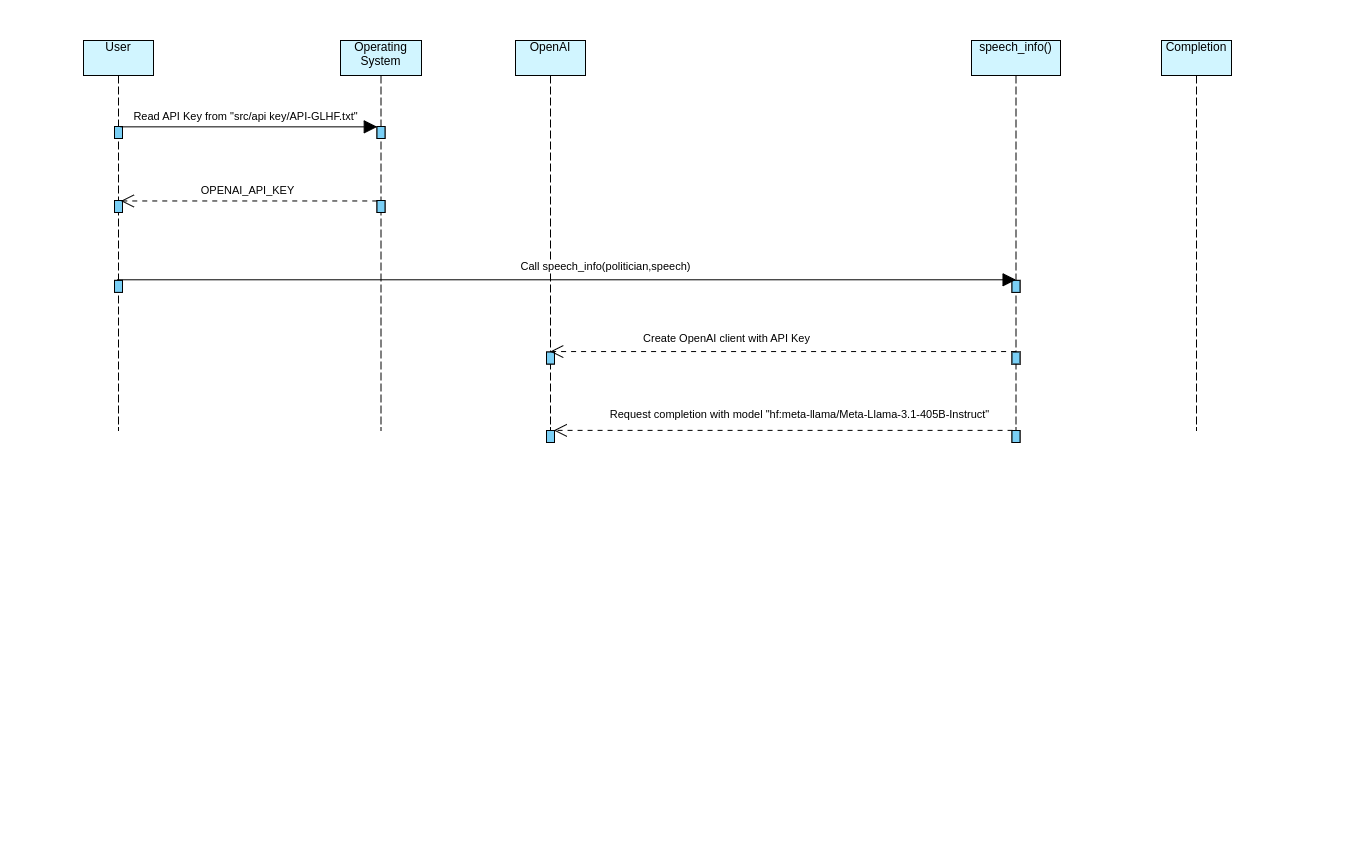
\includegraphics[width=0.8\textwidth]{speechscraping.png}
		\caption{Sequence diagram del processo di speech scraping.}
		\label{fig:speechscraping}
		% Seconda immagine
		\vspace{1em} % Aggiunge spazio tra le immagini
		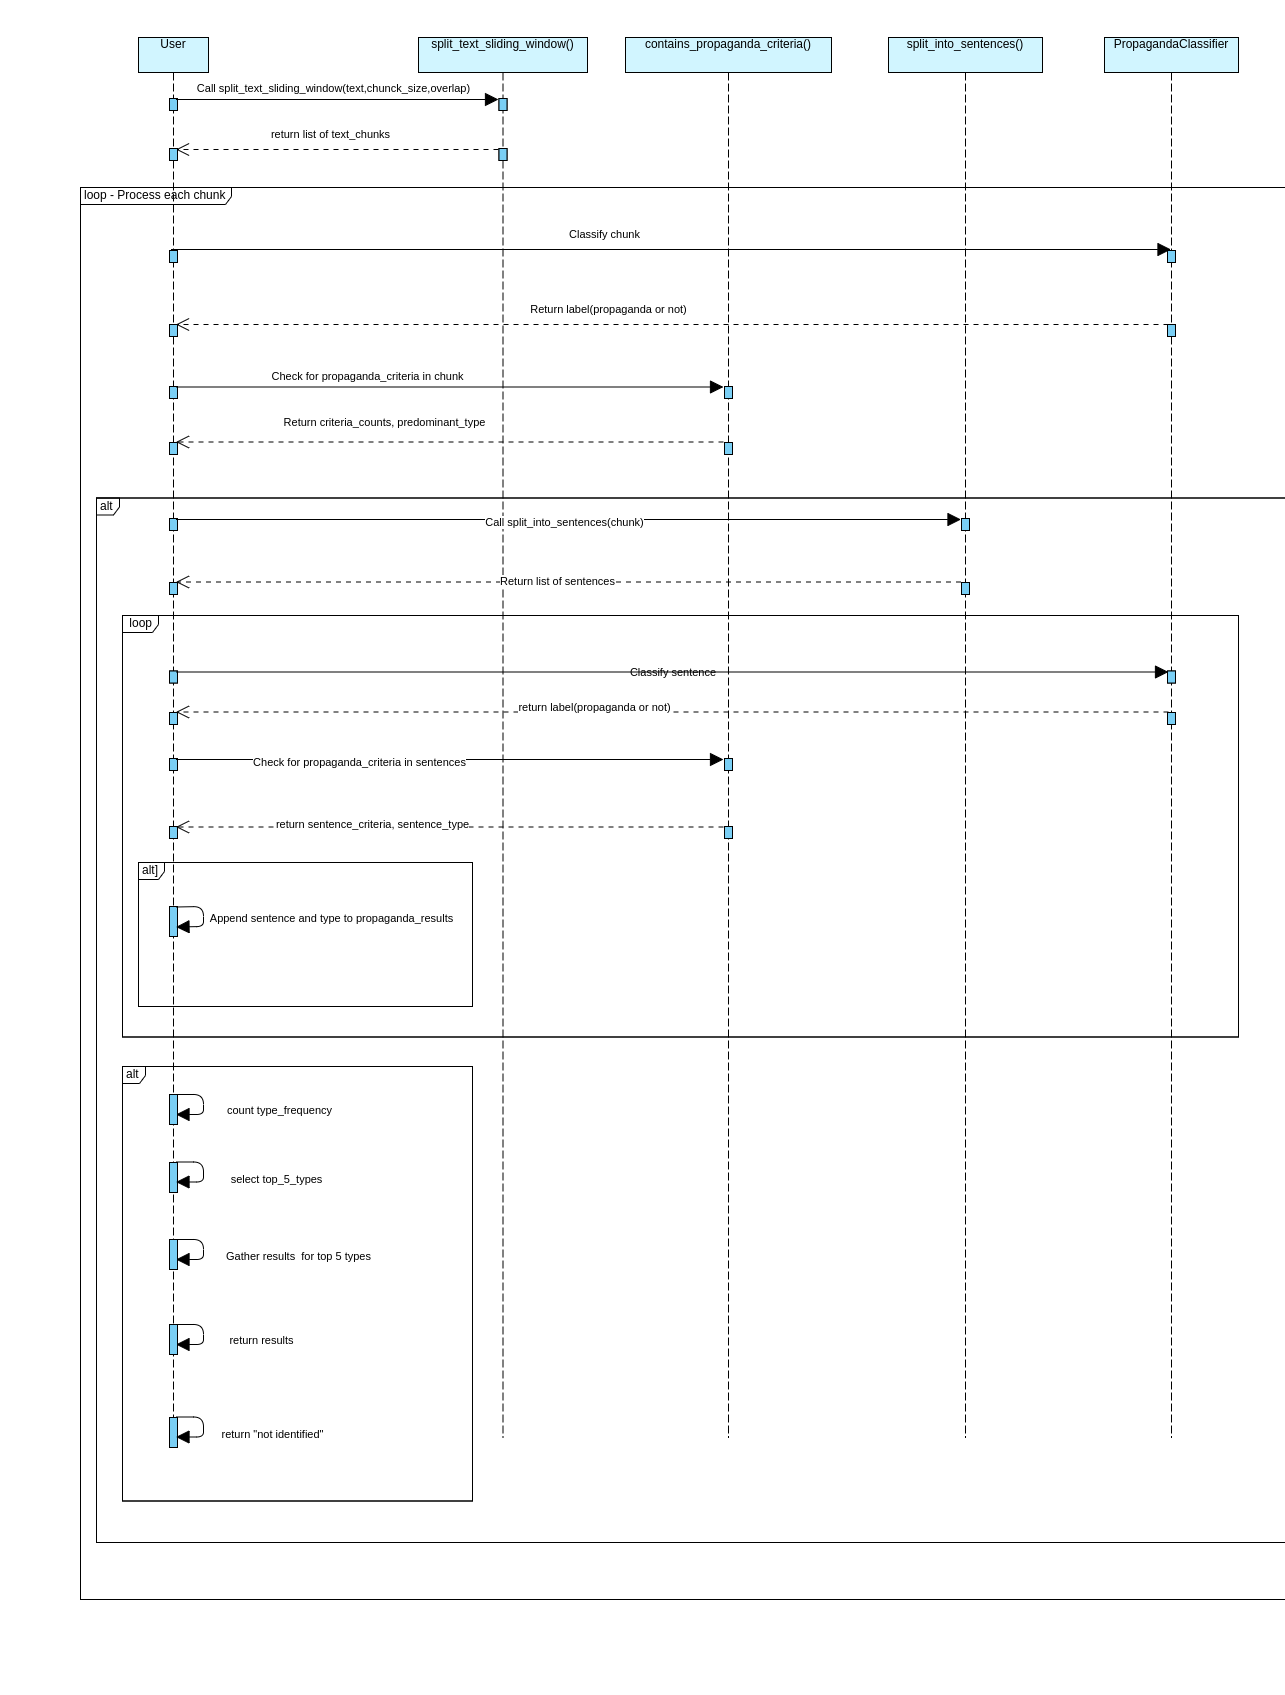
\includegraphics[width=0.8\textwidth]{propagandatype.png}
		\caption{Sequence diagram del processo di propaganda type detection.}
		\label{fig:propagandatype}
		% Terza immagine
		\vspace{1em} % Aggiunge spazio tra le immagini
		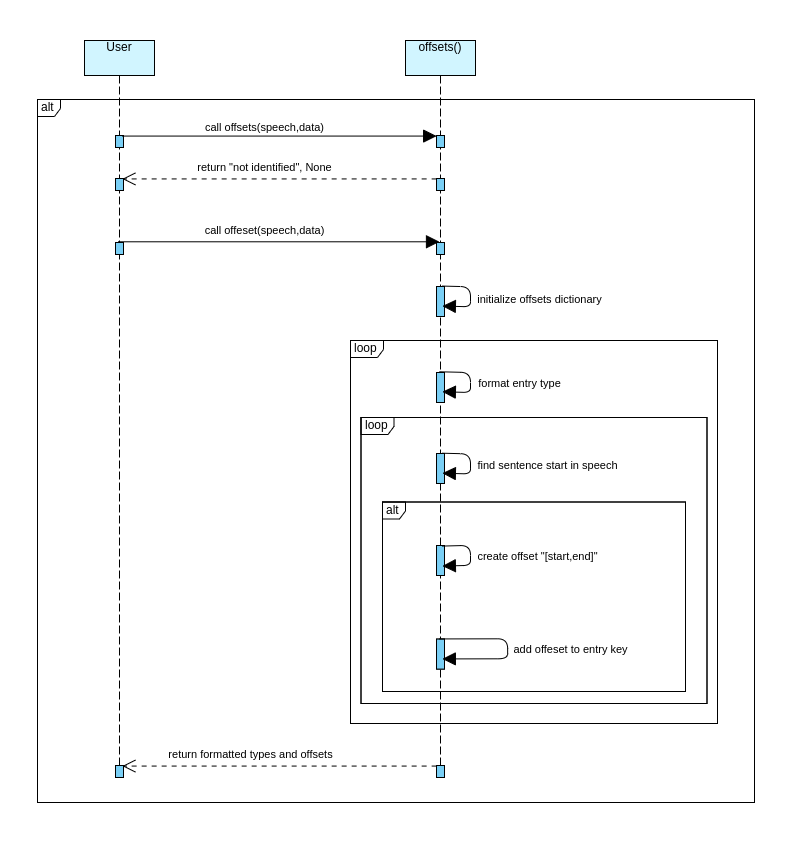
\includegraphics[width=0.8\textwidth]{offset.png}
		\caption{Sequence diagram del processo di individuazione degli offset.}
		\label{fig:offset}
	\end{figure}
\newpage
	\subsection{Funzioni}
		
		\subsubsection{Verify Politician}
La funzione verifica se un dato titolo della pagina web corrisponde a una figura politica. Utilizza il riassunto della prima frase della pagina di Wikipedia e controlla se contiene parole chiave come "who", "politician" o "statesman". Se si verifica un errore di disambiguazione o la pagina non esiste, restituisce False.
		\begin{lstlisting}
def verify_politician(titolo):

	try:
# Prende la prima frase del riassunto della pagina
		summary = wikipedia.summary(titolo, sentences=1)
# Filtra per le parole chiave contenute nella prima frase
		return any(keyword in summary.lower() for keyword in ["who", "politician", "statesman"])

	except (wikipedia.exceptions.DisambiguationError, wikipedia.exceptions.PageError):
		return False
		\end{lstlisting}
		
		\subsubsection{Get Politician Info}
La funzione effettua una ricerca, verifica se il cognome è associato a un politico (tramite verify politician), e scarica l'HTML della pagina per analizzarlo con BeautifulSoup.
Successivamente, in base al parametro richiesto, estrae e restituisce informazioni come nome, data e luogo di nascita, data e luogo di morte, o partito politico. Questi dati vengono salvati nel dizionario per eventuali richieste future.
		\begin{lstlisting}
# Ottiene le informazioni dal polico
def get_info(cognome, parametro):
	# Verifica se il parametro esiste 
	if cognome in politici and parametro in politici[cognome]:
		return politici[cognome][parametro]

	# Verifica se il cognome esiste e crea il dizionario
	elif cognome not in politici:
		politici[cognome] = {}

	# Verifica se il soup non esiste e lo deve creare
	if "soup" not in politici[cognome]:
	# Cerca su wikipedia il cognome dato
	results = wikipedia.search(cognome)

		# Trova l'indice del risultato del politico tramite la funzione verify_politician
		index = next((i for i, result in enumerate(results) if verify_politician(result)), None)

		if index is not None:
			# Prende l'URL della pagina wikipedia
			url = wikipedia.page(results[index]).url

			# Effettua una richiesta GET alla pagina
			response = requests.get(url)
			
			# Verifica se la richiesta ha avuto successo
			if response.status_code == 200:
			# Crea l'oggetto BeautifulSoup per analizzare l'HTML e lo aggiunge dizionario
			politici[cognome]["soup"] = BeautifulSoup(response.text, features="html.parser")
			else:
			print("Errore nella richiesta della pagina:", response.status_code)

	if "soup" in politici[cognome]:
	soup = politici[cognome]["soup"]
	# Trova l'infobox contenente le rows in cui sono presenti diversi dati
	infobox = soup.find("table", {"class": "infobox"}).find_all("tr")
	
	# Cerca il nome
	if parametro == "name":
		# Estrai il nome completo
		name = soup.find("div", {"class": "nickname"}).text

			if name:
				# Aggiunge il nome al dizionario
				politici[cognome]["name"] = name
				# Restituisce il nome
				return name
			return "N/A"

		# Cerca la data di nascita
		elif parametro == "birthday":
			# Estrae la data di nascita
			birth_date = soup.find("span", {"class": "bday"}).text

			if birth_date:
				# Aggiunge la data di nascita al dizionario
				politici[cognome]["birthday"] = birth_date
				# Restituisce la data di nascita
				return birth_date
			return "N/A"

		# Cerca il luogo di nascita
		elif parametro == "birthplace":
			# Trova il luogo di nascita in caso questo sia un link
			try:
				# Estrae il luogo di nascita
				birth_place = next(
				# Prende il link del luogo di nascita e lo unisce allo Stato di nascita
				("%s%s" % (row.find("a").text, row.find("a").find_next_sibling(string=True).text)
				for row in infobox if "Born" in row.get_text()), 
				None
				)
			# Trova il luogo di nascita in caso questo sia una scritta semplice
			except AttributeError:
				# Estrae il luogo di nascita
				birth_place = next(
				# Prende la stringa del luogo di nascita
				("%s" % row.find("br").find_next_sibling(string=True).text
				for row in infobox if "Born" in row.get_text()), 
				None
				)

			if birth_place:
				# Aggiunge il luogo di nascita al dizionario
				politici[cognome]["birthplace"] = birth_place
				# Restituisce il luogo di nascita
				return birth_place
			return "N/A"

		# Cerca la data di morte
		elif parametro == "deathday":
			# Estrae la data di morte
			death_day = next(
				# Prende lo span della data di morte
				(row.find("span").text
				for row in infobox if "Died" in row.get_text()), 
				None
			)	

			if death_day:
				# Riformatta la data per togliere le parentesi ed avere il formato aaaa-mm-gg
				death_day = death_day[1:-1]
				# Aggiunge la data di morte al dizionario
				politici[cognome]["deathday"] = death_day
				# Restituisce la data di morte
				return death_day
			# Aggiunge None al dizionario nel caso in cui la persona non sia morta
			politici[cognome]["deathday"] = None
			return None

		# Cerca il luogo di morte
		elif parametro == "deathplace":
			# Trova il luogo di morte in caso questo sia un link
			try:
				# Estrae il luogo di morte
				death_place = next(
				# Prende il link del luogo di morte e lo unisce allo Stato di morte
				("%s%s" % (row.find("a").text, row.find("a").find_next_sibling(string=True).text)
				for row in infobox if "Died" in row.get_text()), 
				None
			)
			# Trova il luogo di nascita in caso questo sia una scritta semplice
			except AttributeError:
				death_place = next(
				# Prende la stringa del luogo di morte
				("%s" % row.find("br").find_next_sibling(string=True).text
				for row in infobox if "Died" in row.get_text()), 
				None
			)

			if death_place:
				# Aggiunge il luogo di morte al dizionario
				politici[cognome]["deathplace"] = death_place
				# Restituisce il luogo di morte
				return death_place
			# Aggiunge None al dizionario nel caso in cui la persona non sia morta
			politici[cognome]["deathplace"] = None
			return None

		# Cerca il partito politico
		elif parametro == "party":
			# Estrae il partito politico
			party = next(
			# Prende il link del partito politico
				("%s" % row.find("a").text
				for row in infobox if "Political party" in row.get_text()), 
				None
			)

			if party:
				# Aggiunge il partito politico al dizionario
				politici[cognome]["party"] = party
				# Restituisce il partito politico
				return party
			return "N/A"

		else:
			print("Parametro selezionato non valido.")
	
		\end{lstlisting}

		\subsubsection{Speech Info}
La funzione utilizza llama per ottenere varie informazioni sul discorso. Oltre alla data e al luogo in cui si è tenuto il discorso, attraverso il prompt vengono riportati anche l'occasione in cui si è tenuto, il topic di cui tratta, i cognitive bias, una summary e un'analisi dello storytelling.
		\begin{lstlisting}
def speech_info(politician, speech):
	try:
		client = openai.OpenAI(
			api_key=os.environ.get("OPENAI_API_KEY"),
			base_url="https://glhf.chat/api/openai/v1"
		)
		completion = client.chat.completions.create(
			model="hf:meta-llama/Meta-Llama-3.1-405B-Instruct"
			messages=[Prompt]
		temperature=0
		
	return speech, completion.choices[0].message.content
	
	except (openai.RateLimitError, Exception):
	raise
		\end{lstlisting}
\newpage		
		\subsubsection{Speech Data}
		Questa funzione è progettata per estrarre i dati associati a un determinato discorso (speech) da un dizionario (results dict) e formattarli in un array con esattamente 8 valori, gestendo eventuali errori.
		\begin{lstlisting}
def get_speech_data(speech, results_dict):
	try:
		parts = results_dict[speech].split('$')
		parts += ["N/A"] * (8 - len(parts))
		return parts[:8]
	except (KeyError, Exception):
		return ["N/A", "N/A", "N/A", "N/A", "N/A", "N/A", "N/A", "N/A"]

		\end{lstlisting}
		
		\subsubsection{Classify Text}
La funzione classifica un testo in base a un modello pre-addestrato.
	\begin{lstlisting}
# Funzione unificata per classificare il testo
def classify_text(text, model, tokenizer, labels):
inputs = tokenizer(text, return_tensors="pt", truncation=True)
outputs = model(**inputs)
probabilities = torch.nn.functional.softmax(outputs.logits, dim=1)
prediction = torch.argmax(probabilities, dim=1).item()
return labels[prediction].capitalize()	
	\end{lstlisting}
	
		\subsubsection{Split Sentences}
	La funzione suddivide un testo in singole frasi utilizzando una semplice espressione regolare.
	\begin{lstlisting}
# Dividi il testo in frasi usando una semplice regex
def split_into_sentences(text):
	sentence_endings = re.compile(r'(?<=[.!?])\s+')
	return sentence_endings.split(text)
	\end{lstlisting}
	
		\subsubsection{Propaganda Criteria}
La funzione analizza un testo per rilevare la presenza di elementi riconducibili a tecniche di propaganda. Confronta il contenuto del testo con un insieme di parole o frasi chiave definite per ciascun criterio, come toni accusatori, distorsione dell’opposizione o appelli alla paura. Per ogni criterio, conta quante volte le frasi chiave sono presenti nel testo. Se vengono rilevati uno o più criteri, restituisce un dizionario con il conteggio delle occorrenze e il criterio predominante (quello con più corrispondenze). Se non viene rilevato nulla, restituisce `None`.	
	\begin{lstlisting}
# Funzione per rilevare i criteri di propaganda
def contains_propaganda_criteria(text):
	criteria = {
		"accusatory_tone": ["fault of"],
		"opposition_distortion": ["enemies", "traitor", "dishonest", "corrupt"],
		"slogan_repetition": ["you have to believe", "the truth is", "don't forget", "do not forget"],
		"fear_appeals": ["danger", "threat", "crisis", "chaos"],
		"flagwaving": ["our nation", "homeland", "defend values"],
		"black_white_fallacy": ["either with us or against us", "only choice"],
		"clichés": ["golden times", "like once upon a time", "old times"]
	}
	# Conta quante frasi/parole chiave sono presenti per ciascun criterio
	type_counts = {key: sum(phrase in text.lower() for phrase in phrases) for key, phrases in criteria.items()}
	# Filtra i criteri che hanno almeno una corrispondenza
	detected_types = {key: count for key, count in type_counts.items() if count > 0}
	# Se non ci sono criteri rilevati, ritorna None
	if not detected_types:
	return None, None
	predominant_type = max(detected_types, key=detected_types.get)
	return detected_types, predominant_type
	\end{lstlisting}
		
		\subsubsection{Detect Propaganda Type}
La funzione suddivide il testo in chunk sovrapposti per garantire che tutte le parti siano valutate senza perdere contesto. Ogni chunk viene analizzato sia tramite un modello di classificazione di propaganda che con una funzione che cerca criteri definiti di propaganda nel testo. Se un chunk è classificato come propaganda o contiene criteri rilevanti, viene ulteriormente diviso in frasi per un'analisi più dettagliata.\\
Per ciascuna frase classificata come propaganda, vengono salvati il tipo di propaganda identificato e la frase stessa. Infine, se vengono rilevati risultati, la funzione restituisce i cinque tipi di propaganda più comuni, ciascuno accompagnato dalle frasi associate. Se non viene rilevato nulla, restituisce "Not identified".	
	\begin{lstlisting}
def detect_propaganda_type(text, classifier=propaganda_classifier, chunk_size=512, overlap=128):
	# Divide il testo in chunk
	text_chunks = split_text_sliding_window(text, chunk_size, overlap)
	propaganda_results = []

	for chunk in text_chunks:
		# Classifica il chunk
		is_propaganda_by_model = classifier(chunk, truncation=True, max_length=chunk_size)[0]['label'] == "propaganda"
		criteria_counts, predominant_type = contains_propaganda_criteria(chunk)

		# Analizza le frasi del chunk
		if is_propaganda_by_model or criteria_counts:
			sentences = split_into_sentences(chunk)  # Dividi il chunk in frasi
			for sentence in sentences:
				# Classifica la singola frase
				sentence_is_propaganda = classifier(sentence, truncation=True)[0]['label'] == "propaganda"
				sentence_criteria, sentence_type = contains_propaganda_criteria(sentence)
				
				if sentence_is_propaganda or sentence_criteria:

					propaganda_results.append({
						"type": sentence_type,
						"sentence": sentence
					})

	# Se esistono risultati di propaganda
	if propaganda_results:
		# Conta la frequenza di ogni tipo di propaganda
		types = [result["type"] for result in propaganda_results]
		type_counts = Counter(types)

		# Prendi le 5 tipologie più comuni
		top_5_types = type_counts.most_common(5)

		# Estrai i risultati per le 5 tipologie più comuni
		results = []
		for propaganda_type, _ in top_5_types:
			sentences_of_type = [
			{"sentence": result["sentence"]}
			for result in propaganda_results if result["type"] == propaganda_type
			]
			results.append({
				"type": propaganda_type,
				"sentences": sentences_of_type
			})
			
			return results
			
		return "Not identified"

	\end{lstlisting}
	
		\subsubsection{Contains Toxicity Criteria}

La funzione analizza un testo per identificare criteri di tossicità basati su un insieme di categorie predefinite. Ogni categoria, come insulti, minacce o linguaggio violento, è associata a una lista di parole o frasi chiave indicative di quella forma di tossicità.\\
Confronta il testo con le chiavi, calcola il numero di corrispondenze per ciascuna categoria, e restituisce un dizionario con i criteri rilevati e il loro conteggio. Inoltre, identifica quale categoria è predominante, ovvero quella con il maggior numero di corrispondenze. Se nessun criterio è rilevato, restituisce None.
	\begin{lstlisting}
# Funzione per rilevare i criteri di tossicità
def contains_toxicity_criteria(text):
	criteria = {
		"insults": ["idiot", "stupid", "moron", "fool", "scum", "loser", "crooked", "degenerate", "ignoramus"],
		"threats": ["destroy", "kill", "eliminate", "eradicate", "you'll regret", "annihilate", "purge", "defeat utterly"],
		"violent_language": ["blood", "war", "fight", "smash", "knock them out", "battle", "no quarter"],
		"divisive_statements": ["us vs them", "enemy of the people", "deep state", "traitors", "fifth column"],
		"personal_attacks": ["you always fail", "your fault", "worthless", "incompetent", "phony", "betrayer"],
		"exaggerations": ["always lie", "never truthful", "the worst", "greatest challenge", "unprecedented threat"],
		"fear_appeals": ["danger", "threat", "crisis", "chaos", "they're coming for you", "crime wave"],
			"flagwaving": ["our nation", "homeland", "defend values", "make america great again", "fatherland", "motherland", "maga"]
	}
	# Conta quante frasi/parole chiave sono presenti per ciascun criterio
	type_counts = {key: sum(phrase in text.lower() for phrase in phrases) for key, phrases in criteria.items()}
	# Filtra i criteri che hanno almeno una corrispondenza
	detected_types = {key: count for key, count in type_counts.items() if count > 0}
	# Se non ci sono criteri rilevati, ritorna None
	if not detected_types:
		return None, None
	# Identifica il tipo di tossicità
	predominant_type = max(detected_types, key=detected_types.get)
	return detected_types, predominant_type
	\end{lstlisting}
	
		\subsubsection{Classify Toxicity}
La funzione  classifica un testo identificando eventuali criteri di tossicità. Utilizza la funzione contains toxicity criteria per analizzare il testo e determinare quali categorie di tossicità sono presenti, insieme al conteggio delle loro occorrenze.
Se vengono rilevati criteri, questi vengono formattati come una lista leggibile in cui ogni riga mostra il nome del criterio (con spazi al posto degli underscore) e il numero di volte che è stato riscontrato.
	\begin{lstlisting}
# Funzione per classificare la tossicità
def classify_toxicity(text):
	try:
		# Rilevamento criteri
		detected_criteria, _ = contains_toxicity_criteria(text)

		# Formattare i criteri rilevati uno per riga
		if detected_criteria:
			return '\n'.join(["%s: %s" % (k, v) for k, v in detected_criteria.items()]).replace("_", " ").title()
		else:
			return ""
	except Exception:
		raise
	\end{lstlisting}
	
		\subsection{Offsets}	
La funzione calcola gli offset delle frasi identificate come propaganda all'interno di un discorso, fornendo la posizione iniziale e finale di ogni frase rilevata per ciascun tipo di propaganda attraverso il formato [inizio:fine].
Se il parametro data contiene il valore "Not identified", la funzione restituisce direttamente questo valore con None, indicando che non sono state rilevate frasi di propaganda.		
	\begin{lstlisting}
def offsets(speech, data):

	# Verifica che la propaganda sia stata correttamente identificata
	if data == "Not identified":
		return "Not identified", None

	# Crea un dizionario per definire gli offset
	offsets = {
		# Crea una chiave per tipo e la formatta correttamente 
		entry["type"].replace("_", " ").capitalize(): [
			# Crea un offset per ogni frase
			"[%s:%s]" % (start, start + len(sentence["sentence"]))
			for sentence in entry["sentences"]
			# Trova le frasi e le misura
			if (start := speech.find(sentence["sentence"])) != -1
		]
	for entry in data
}

	# Restituice il tipo di propaganda e gli offset per ogni tipo di propaganda
	return "\n".join(offsets.keys()), "\n".join("%s: %s" % (key, ", ".join(element)) for key, element in offsets.items())
	\end{lstlisting}
	
		\subsubsection{Formality}
La funzione determina se un discorso è formale o informale in base al suo livello di soggettività utilizzando il modulo TextBlob per analizzare il sentiment del testo. Se la lunghezza del discorso è inferiore o uguale a 150 caratteri, la funzione restituisce "N/A", indicando che la valutazione non è applicabile.\\
Se il discorso è più lungo, la funzione analizza la soggettività del testo: una soggettività inferiore a 0,5 suggerisce che il testo è formale, mentre una soggettività più alta indica che il discorso è informale.	
	\begin{lstlisting}
def is_formal(speech):
	if len(speech) <= 150:
		return "N/A"
	
	blob = TextBlob(speech)
	# Bassa soggettività indica formalità
	if blob.sentiment.subjectivity < 0.5:
		return "Formal"
	else:
		return "Informal"
	\end{lstlisting}
	
		\subsubsection{Leggibilità}
La funzione calcola diverse metriche di leggibilità di un discorso utilizzando il modulo textstat, che fornisce diversi indici per valutare quanto sia facile o difficile leggere un testo. Le metriche prese in considerazione sono: flesch reading ease, flesch-kincaid grade, gunning fog, SMOG index.
	\begin{lstlisting}
# Funzione per calcolare metriche di leggibilità
def calcola_legibilita(speech):
	return {
		"flesch_reading_ease": textstat.flesch_reading_ease(speech), # facilità di lettura basandosi sulla lunghezza delle frasi e sul numero di sillabe per parola
		"flesch_kincaid_grade": textstat.flesch_kincaid_grade(speech), #  anni di istruzione necessari per comprendere il testo
		"gunning_fog": textstat.gunning_fog(speech), # complessità del speech in base alla lunghezza delle frasi e alla percentuale di parole complesse
		"smog_index": textstat.smog_index(speech), # come quello precedente
		"text_standard": textstat.text_standard(speech) # sintetizzazione dei risultati in un livello scolastico approssimativo
	}
	\end{lstlisting}
	
		\subsubsection{Analyze Narrative Structure}
La funzione analizza la struttura narrativa di un discorso, concentrandosi su vari aspetti legati alla lunghezza e alla variabilità delle frasi. In seguito alla tokenizzazione, viene calcolato il numero di parole all'interno di ogni token, generando una lista che rappresenta la lunghezza di ogni frase.
Dopo aver ottenuto le lunghezze delle frasi, la funzione calcola diverse metriche narrative. La lunghezza media delle frasi viene determinata calcolando la media aritmetica del numero di parole per ciascuna frase. Viene poi calcolata la deviazione standard, che misura quanto le lunghezze delle frasi variano l'una dall'altra, dando un'idea della coerenza o della varietà nella struttura del discorso. Inoltre, la funzione conta il numero totale di frasi nel discorso e, infine, calcola un punteggio di complessità, che è il rapporto tra la lunghezza media delle frasi e la deviazione standard.		
	\begin{lstlisting}
def analyze_narrative_structure(speech):
	sentences = sent_tokenize(speech)
	
	# Analyze sentence length variation
	sentence_lengths = [len(sentence.split()) for sentence in sentences]
	
	narrative_metrics = {
		'Average Sentence Length': np.mean(sentence_lengths),
		'Sentence Length Variation': np.std(sentence_lengths),
		'Total Sentences': len(sentences),
		'Complexity Score': np.mean(sentence_lengths) / (np.std(sentence_lengths) + 1)
	}

	return "\n".join(["%s: %.3f" % (key, value) if isinstance(value, float) else "%s: %d" % (key, value) for key, value in narrative_metrics.items()])

	\end{lstlisting}
			
			\subsubsection{TF-IDF}
La funzione estrae le parole chiave più rilevanti da un discorso utilizzando il metodo TF-IDF. Imposta un limite sul numero di parole chiave da restituire (top 5) e ignora le stop words. Successivamente, calcola la matrice TF-IDF e seleziona le parole con i punteggi più alti. Le parole chiave e i loro punteggi vengono quindi ordinati e restituiti in una stringa formattata con i punteggi arrotondati a tre decimali, mettendo in evidenza le parole più significative nel testo.	
	\begin{lstlisting}	
def tfidf(speech):
	# Definisce il numero di parole massimo per le keywords
	max_ngram_length = 1
	# Definisce quante keywords dobbiamo trovare
	top_n = 5

	# Inserisce i parametri di ricerca e il dizionario delle stop words
	vectorizer = TfidfVectorizer(
		ngram_range=(1, max_ngram_length),
		stop_words='english'
	)

	# Prende la matrice TF-IDF
	tfidf_matrix = vectorizer.fit_transform([speech])
	
	# Prende i nomi delle parole
	feature_names = vectorizer.get_feature_names_out()
	
	# Prende gli score TF-IDF
	tfidf_scores = tfidf_matrix.toarray()[0]

	# Crea una lista di tuple (keyword, score)
		keyword_scores = [
		(feature_names[idx], score)
		for idx, score in enumerate(tfidf_scores)
		if score > 0
	]

	# Ordina per score decrescente
	keyword_scores = sorted(keyword_scores, key=lambda x: x[1], reverse=True)
	
	# Prende solo le top_n keywords
	top_keywords = keyword_scores[:top_n]
	
	# Restituisce le parole chiave con i rispettivi punteggi
	return "\n".join(["%s: %.3f" % (kw.title(), round(score, 3)) for kw, score in top_keywords])

	\end{lstlisting}

		\subsubsection{Word Embeddings}
La funzione calcola gli embeddings di un testo suddividendolo in chunk di dimensione specificata, con un sovrapposizione tra i chunk. Per ogni chunk, il testo viene tokenizzato e passato attraverso il modello per ottenere gli embeddings dei token. Gli embeddings di ogni token nel chunk vengono mediati (calcolando la media dei vettori) per ottenere un embedding complessivo per il chunk. Alla fine, gli embeddings medi di tutti i chunk vengono mediati nuovamente per ottenere un embedding finale che rappresenta l'intero testo.		
	\begin{lstlisting}
# Funzione per calcolare gli embeddings sui chunk
	def calcola_embedding(testo, tokenizer, model, chunk_size=512, overlap=128):
	chunks = split_text_sliding_window(testo, chunk_size=chunk_size, overlap=overlap)
	embeddings_chunk = []
	
	for chunk in chunks:
		inputs = tokenizer(chunk, return_tensors="pt", padding=True, truncation=True, max_length=chunk_size)

		with torch.no_grad():
			outputs = model(**inputs)

		token_embeddings = outputs.last_hidden_state
		mean_embedding = token_embeddings.mean(dim=1).squeeze()
		embeddings_chunk.append(mean_embedding.cpu().numpy())

	if embeddings_chunk:
		final_embedding = np.mean(embeddings_chunk, axis=0)
	else:
		final_embedding = np.zeros(model.config.hidden_size)
		
	return final_embedding
	\end{lstlisting}
	
		\subsubsection{Visualize Embeddings}
La funzione utilizza i word embedding per creare uno scatter plot in cui ogni punto (enumerato) rappresenti un discorso e ogni colore un politico. Discorsi semanticamente simili saranno altrettanto vicini sul grafico, discorsi semanticamente differenti verranno rappresentati più distanti.
	\begin{lstlisting}
# Visualizza gli embeddings su scatter plot
	def visualize_embeddings(dataset, plt_show, output_path="word_embending.png"):
	tokenizer = AutoTokenizer.from_pretrained("sentence-transformers/all-MiniLM-L6-v2")
	model = AutoModel.from_pretrained("sentence-transformers/all-MiniLM-L6-v2")
	
	dataset["Embedding"] = dataset["Speech"].fillna("").apply(lambda x: calcola_embedding(x, tokenizer, model))
	embeddings = np.stack(dataset["Embedding"].values)
	
	tsne = TSNE(n_components=2, random_state=42, perplexity=30)
	embeddings_2d = tsne.fit_transform(embeddings)
	
	dataset["x"] = embeddings_2d[:, 0]
	dataset["y"] = embeddings_2d[:, 1]
	
	politici_unici = dataset["Surname"].unique()
	
	# Crea una figura di dimensioni (10, 6) e posiziona i punti in base ai nomi
	plt.figure(figsize=(10, 6))
		for politico in politici_unici:
		subset = dataset[dataset["Surname"] == politico]
		plt.scatter(subset["x"], subset["y"], label=politico, alpha=0.7)

	# Enumera ogni discorso sui punti 
	for i, (x, y) in enumerate(zip(dataset["x"], dataset["y"])):
		plt.text(x, y, str(i), fontsize=6, ha='right', va='bottom', color='black', alpha=0.6)

	# Impostazioni del grafico (titolo, label di ascissa e ordinate, leggenda e layout finale)
	plt.title("Embeddings per Politico", fontsize=12)
	plt.xlabel("Asse X", fontsize=10)
	plt.ylabel("Asse Y", fontsize=10)
	plt.legend(title="Politico", bbox_to_anchor=(1.02, 1), loc="upper left", fontsize=8)
	plt.tight_layout()
	# Salva il grafico nella stessa directory del file Python
	plt.savefig(output_path, dpi=300, bbox_inches='tight')
	# Chiudi il plot per evitare conflitti in future visualizzazioni
	
	if plt_show == "s":
		return plt
	
	plt.close()
	return None
	\end{lstlisting}
		
		\subsubsection{Analyze Persuasion}
La funzione analizza un testo per valutare la presenza di elementi persuasivi. Usa spaCy per elaborare il testo e calcolare il numero di superlativi, domande retoriche, e parole emotive, di urgenza, autorità e prova sociale. Ogni metrica è normalizzata in base alla frequenza nel testo e ponderata con un peso specifico che riflette l'importanza persuasiva di ciascun elemento. Somma gli score normalizzati per ottenere un punteggio totale di persuasione. I risultati vengono restituiti in un formato leggibile, con ogni metrica e il suo valore separati da una riga.	
	\begin{lstlisting}
def analyze_persuasion(text):
	# Analisi del testo usando spaCy
	doc = nlp(text.lower())
	
	# Calcola metriche persuasive
	# Per ogni tipo di elemento persuasivo, conta quante volte appare nel testo 
	metrics = {
			# conta i superlativi
			"superlatives": sum(1 for token in doc if token.tag_ in ["JJS", "RBS"]),
			# conta le domande retoriche, basandosi sul fatto che terminano con un punto di domanda
			"rhetorical_questions": sum(1 for sent in doc.sents if sent.text.strip().endswith("?")),
			# conta le parole emotive che appartengono alla lista predefinita
			"emotional_words": sum(1 for token in doc if token.text in PERSUASIVE_WORDS["emotional"]),
			# conta le parole legate all'urgenza dalla lista predefinita
			"urgency_words": sum(1 for token in doc if token.text in PERSUASIVE_WORDS["urgency"]),
			# conta le parole legate all'autorità
			"authority_words": sum(1 for token in doc if token.text in PERSUASIVE_WORDS["authority"]),
			# conta le parole di prova sociale
			"social_proof_words": sum(1 for token in doc if token.text in PERSUASIVE_WORDS["social_proof"])
	}

	# Calcola il numero totale di token
	total_tokens = len(doc)
	# Se il testo non contiene token, restituisce un dizionario vuoto
	if total_tokens == 0:
		return {key: 0.0 for key in metrics.keys() | {"total_score"}}

	# Definisce il peso per ogni elemento persuasivo, indicando quanto è importante ciascuna metrica
	weights = {
		"superlatives": 1.5, # peso medio
		"rhetorical_questions": 2.0, # sono più persuasive
		"emotional_words": 2.5, # sono le più persuasive
		"urgency_words": 2.0, # sono persuasive 
		"authority_words": 1.8, # peso medio-alto
		"social_proof_words": 1.7 # peso inferiore
	}

	# Calcola uno score normalizzato per ogni metrica
	# Per ogni metrica:
	# - Divido il conteggio per il numero totale di token (normalizzazione)
	# - MOltiplico per il peso associato per enfatizzare la sua importanza 
	normalized_scores = {
		key: (metrics[key] / total_tokens) * weights[key] for key in metrics
	}

	# Somma tutti gli score normalizzati per ottenere lo score totale di persuasione
	total_score = sum(normalized_scores.values())
	normalized_scores["total_score"] = round(total_score, 3) # arrotondare a 3 - scelta comune per rappresentare valori numerici in cui la precisione oltre il millesimo non è necessaria
	
	return '\n'.join("%s: %s" % (k.replace('_', ' ').title(), v) for k, v in normalized_scores.items()) # restituisce gli score
	\end{lstlisting}
	
	\subsection{Esempio d'uso}

\newpage
	\textsc{\large METTI FOTO}\\[0.2cm]
\section{Analisi delle Prestazioni}
	\subsection{Metriche}
	\subsection{Limiti identificati}

\newpage
\section{Conclusioni}
Il team è riuscito a completare con successo il project work assegnato grazie a una solida collaborazione, una gestione efficace del tempo e un'accurata pianificazione delle attività.  La continua iterazione, brainstorming e testing dei modelli hanno permesso di superare le difficoltà tecniche iniziali dovute alla novità della richiesta e rispettare i tempi stabiliti. Alla fine, il lavoro è stato completato con il raggiungimento degli obiettivi prefissati in modo soddisfacente.

\section{Appendice}
\subsection{GitHub}
\end{document}